\documentclass[11pt]{article}
\usepackage{fullpage}
\usepackage{graphicx}
\title{Sistema de Inferencia de L\'ogica Difusa GFIS}
\author{Ariel Coto Santiesteban C412}
\begin{document}
\maketitle
\section{Caractr\'isticas del Sistema}
\textbf{GFIS} permite resolver cualquier problema de inferencia si desea implementarse un sistema de soluciones basado en L\'ogica Difusa, en \emph{Python 3}. Para esto, se le ofrece al usuario dos clases fundamentales, \textbf{MemberFunct} y \textbf{DiffSystem}.
\subsection{Funciones de Membres\'ia}
Un paso crucial para crear un sistema de soluciones basado en l\'ogica difusa, es definirse los par\'ametros de entrada al sistema y todas las posibles clasificaciones de cada entrada. Por ejemplo, como par\'ametro de entrada, la \emph{Temperatura} en grados celcius, y clasificaciones: \emph{Alta}, \emph{Baja} y \emph{Media}. En \textbf{GFIS} para poder definirse estas funciones de membrec\'ia, se utiliza la clase \textbf{MemberFunct}. Una limitaci\'on es que solo se pueden crear funciones trapezoidales y triangulares. Como entrada se le debe aclarar los nombres de a cu\'al par\'ametro define (\emph{Temperatura} o \emph{Presi\'on}, u otra cosa), y el nombre de la funci\'on de membres\'ia a la cual va a describir sobre ese par\'ametro (\emph{Alta}, \emph{Baja}, etc). Adem\'as, debe seleccionar el tipo de funci\'on que desea (trapezoidal o triangular) y los puntos que describen a esta. Se le puede pasar, por \'ultimo, la funci\'on de membres\'ia directamente, la cual debe recibir un entero y devolver otro, pero se recomienda pasarle \textit{None} a esta entrada. \\
\subsection{Sistema y operaciones}
Luego de creadas las funciones de membres\'ia, se pasa a configurar al sistema que incorpora todas las funciones. Para ello se ofrece la clase \textbf{DiffSystem}. A la hora de instanciar el sistema, se debe definir como entrada un diccionario que mapee de la forma 
 \textit{(\textless Nombre\_Campo\textgreater,\textless Nombre\_F\_Mebrec\'ia\textgreater): \textless funci\'on\_de\_membrec\'ia\textgreater}. Ejemplo: \textit{('Temperatura','Alta'): \textless objeto-funci\'on\textgreater}. Seguidamente, se pasa a definir las reglas del sistema.\\
  \textbf{GFIS} le ofrece, en la clase \textbf{DiffSystem}, las operaciones \emph{fuzzy\_and}, \emph{fuzzy\_or} y \emph{fuzzy\_not}. Para obtener una secuencia de operaciones, el usuario debe componer, seg\'un el orden operacional que desee, estas funciones. Una entrada simple a una operaci\'on se define con un string con la forma: \emph{\textless Nombre\_del\_campo\textgreater \textless espacio\textgreater \textless Nombre\_f\_membrec\'ia\textgreater}, llam\'emosle \emph{entrada simple}. Ejemplo: \emph{Temperatura Alta}. Con las operaciones \emph{and}, \emph{or} y \emph{not}, se crea el cuerpo del \emph{if} de la regla. Para a\~nadir la regla al sistema se utiliza la funci\'on \emph{add\_rule} de la clase \textbf{DiffSystem}, que recibe como primer par\'ametro el cuerpo del \emph{if} y como segundo par\'ametro un string como la \emph{entrada simple}, que representa el cuerpo del \emph{then} de la regla.
 \subsection{La salida}
 Para obetener la salida del sistema, se hace a trav\'es de la funci\'on \emph{get\_output} de la clase \textbf{DiffSystem}. Esta recibe como par\'ametros un diccionario que mapea de nombre de los campos medidos a medici\'on, el nombre de la funci\'on de inferencia a utilizar, el nombre de la funci\'on de desifusificaci\'on, y si desea plotear la funci\'on resultante.
 La salida es un entero con el valor de la inferencia, y una lista con los resultados de las evaluaciones de las reglas.
 Los m\'etodos de inferencia disponibles son: \emph{mamdani} y \emph{larsen}.
 Los m\'etodos de desifusificaci\'on disponibles son: \emph{lom}, \emph{som}, \emph{mom}, \emph{centroid} y \emph{bisec}.

\section{Principales ideas sobre la implementaci\'on}
\subsection{Clase MemberFunct}
Esta clase es la interfaz que se ofrece para crear las funciones de membres\'ia de las caracter\'isticas del sistema. La clase posee una funci\'on \emph{evaluate}, que ser\'a la que devuelva la evaluaci\'on sobre la funci\'on. Inicialmente tiene la forma:
\begin{equation}
	\max(\min(\frac{(x - a)}{(b - a)}, \frac{(c - x)}{(c - b)}), 0),
\end{equation}
en el caso de ser triangular con puntos en $a,b$ y $c$; y si es trapezoidal

\begin{equation}
		f(x) = \left\{
		\begin{array}{1cc}
			\max(\min(\frac{(x - a)}{(b - a)},1 , \frac{(d - x)}{(d - c)}), 0)  & si & b-a\neq 0,\\
		\\\max(\min(1 , \frac{(d - x)}{(d - c)}), 0)  & si & b-a = 0,\\
		
		\end{array}
		\right.
\end{equation}
puesto que $d$ y $c$ se asume que siempre ser\'an distintos de cero. Esta clase tiene redefinido el m\'etodo \emph{\_\_add\_\_} para mezclar dos funciones de membres\'ia, cuya implementaci\'on basicamente es devolver un nuevo objeto cuya funci\'on \emph{evaluate} es 
\begin{equation}
	lambda\; x: \max(member\_function1.evaluate(x), member\_function2.evaluate(x)).
\end{equation}

\subsection{Clase DiffSystem}
Esta es la clase fundamental que se le ofrece al usuario para encajar todas las piezas del sistema. Todas las funciones de membres\'ia se pasan en la inicializaci\'on de la clase. Simulando el patr\'on Factory, para acceder a una funci\'on de membres\'ia se hace a trav\'es de la funci\'on \emph{get\_member\_func}, la cual devuelve una nueva instancia de esa funci\'on. Su funci\'on principal es \emph{get\_output} que devuelve el resultado de inferencia del sistema junto a los resultados de evaluar cada regla. Esta funci\'on lo que hace basicamente es:
\begin{enumerate}
	\item Guardar el \emph{input\_data} y resolver las funciones de inferencia y desifusificaci\'on.
	\item Evaluar las reglas del sistema. Agrupar las que tengan igual consecuente y se escoge la de mayor valor de evaluaci\'on para cada consecuente distinto.
	\item Se aplica la funci\'on de inferencia a cada regla, y se agregan todas las funciones.
	\item A la resultante se le aplica el m\'etodo de desifusificaci\'on escogido.
	\item Se devuelve el resultado.
\end{enumerate}
\subsection{Las reglas}
Para las operaciones \emph{and}, \emph{or} y \emph{not} sobre las funciones de membres\'ia, es obligado utilizar las funciones \emph{fuzzy\_and}, \emph{fuzzy\_or} y \emph{fuzzy\_not} de la clase \textbf{DiffSystem}. Estas son funciones que capturan los par\'ametros de entrada y devuelven otra funci\'on que ser\'a la que eval\'ue la regla. La evaluaci\'on se resuelve en profundidad.
\subsection{C\'odigo}
Las clases que se ofrecen se encuentran en el archivo \emph{fuzzySys.py}. Si desea utilizarlas debe importarlas de all\'i. Adem\'as, se ofrece un ejemplo de c\'omo utilizar el sistema en el archivo \emph{example.py}.

\section{Propuesta de Problema a solucionar}
Dado un televisor que detecta si hay ruido en el ambiente y el volumen de la se\~nal, determina si subir o bajar el volumen. (Se desconocen las m\'etricas reales del problema). Se desea saber en cada momento en qu\'e estado dejar el volumen del televisor. Supongamos que el Ruido tiene 3 categor\'ias:
\begin{enumerate}
	\item Bajo (trapezoidal que comienza con (0,1), (50,1), (60,0))
	\item Medio (trapezoidal que comienza con (50,0),(60,1),(80,1),(90,0))
	\item Alto (trapezoidal que comienza con (80,0), (90,1), ($\infty$,1)),
\end{enumerate}
(ver figura \ref{fig:ruido}),
\begin{figure}[ht]
	\centering
	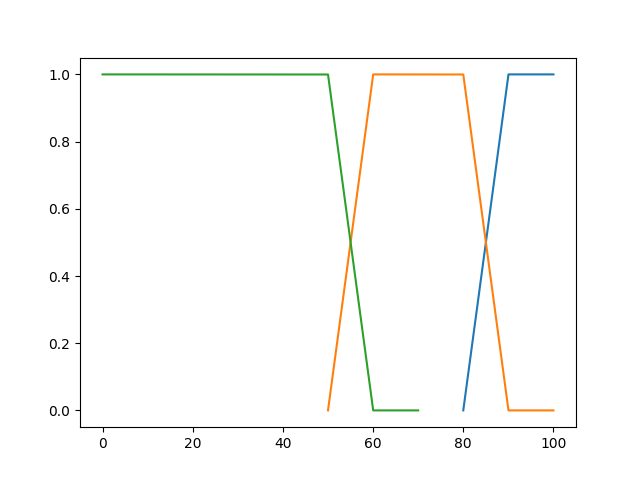
\includegraphics[width=.5\textwidth]{images/Ruido.png}			
	\caption{Categor\'ias del Ruido:  Bajo(verde), Medio(Naranja) y Alto(azul).}
	\label{fig:ruido}	
\end{figure}
 y que el volumen de la se\~nal tenga como categor\'ias
\begin{enumerate}
	\item Bajo (trapezoidal que comienza con (0,1), (50,1), (60,0))
	\item Medio (triangular que comienza con (50,0),(70,1),(90,0))
	\item Alto (trapezoidal que comienza con (70,0), (90,1), ($\infty$,1))
\end{enumerate}
(ver figura \ref{fig:volSig}).\\
\begin{figure}[ht]
	\centering
	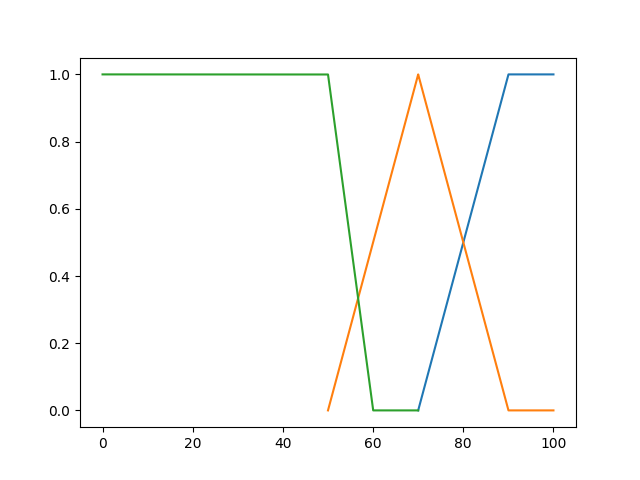
\includegraphics[width=.5\textwidth]{images/VolumenDeLaSignal.png}			
	\caption{Categor\'ias del Volumen de la Se\~nal:  Bajo(verde), Medio(Naranja) y Alto(azul).}
	\label{fig:volSig}	
\end{figure}

El volumen del televisor tiene como categor\'ias:
\begin{enumerate}
	\item Bajo (trapezoidal que comienza con (0,1), (5,1), (10,0))
	\item Medio (triangular que comienza con (5,0),(10,1),(15,0))
\end{enumerate}
(ver figura \ref{fig:volTV}).
\begin{figure}[ht]
	\centering
	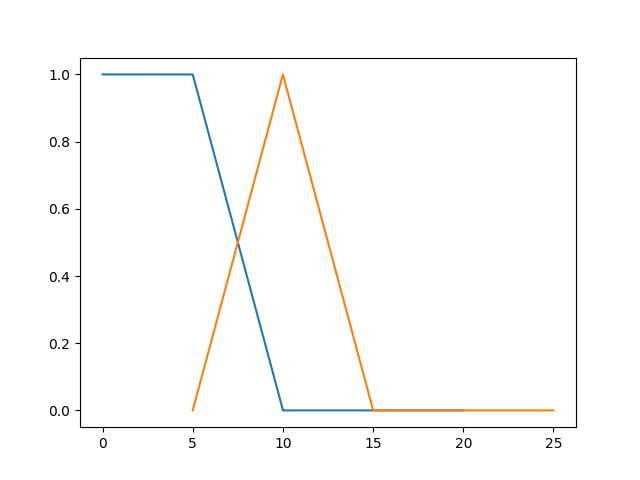
\includegraphics[width=.5\textwidth]{images/VolumenDeLaTV.png}			
	\caption{Categor\'ias del Volumen de la TV:  Bajo(azul) y Medio(Naranja).}
	\label{fig:volTV}	
\end{figure}

 \subsection{Reglas del problema}
Se propuso al problema el siguiente conjunto de reglas:
\begin{itemize}
	\item \textbf{IF} Ruido Alto \textbf{OR} VolumenDeLaSe\~nal Alto \textbf{THEN} VolumenDeLaTV Bajo
	\item \textbf{IF} Ruido Alto \textbf{AND} (\textbf{NOT VolumenDeLaSe\~nal Alto}) \textbf{THEN} VolumenDeLaTV Medio
	\item \textbf{IF} Ruido Medio \textbf{AND} (\textbf{NOT VolumenDeLaSe\~nal Alto}) \textbf{THEN} VolumenDeLaTV Medio
	\item \textbf{IF} Ruido Bajo \textbf{AND} VolumenDeLaSe\~nal Medio \textbf{THEN} VolumenDeLaTV Bajo
	\item \textbf{IF} Ruido Bajo \textbf{AND} VolumenDeLaSe\~nal Bajo \textbf{THEN} VolumenDeLaTV Medio
	
\end{itemize}

\subsection{Resultados del problema}
Este problema est\'a modelado en el archivo \emph{example.py}. Si desea ejecutarlo corra el comando \emph{python3 example.py}. 
Para validar el sistema se prob\'o como entrada $Ruido=87$ y $VolumenDeLaSig=80$, \emph{mandani} como m\'etodo de inferencia y \emph{mom} de desifusificador. Se obtuvo como resultado $7.5$ y como funci\'on resultante la figura \ref{fig:result}. Se interpreta que con un 87 de ruido, que se considera alto, y un 80 de volumen de la se\~nal, que tambi\'en se considera alto, se debe poner el volumen de la TV a 8, redondeando por exceso, dado que la unidad de volumen de un televisor es discreto.


\begin{figure}[ht]
	\centering
	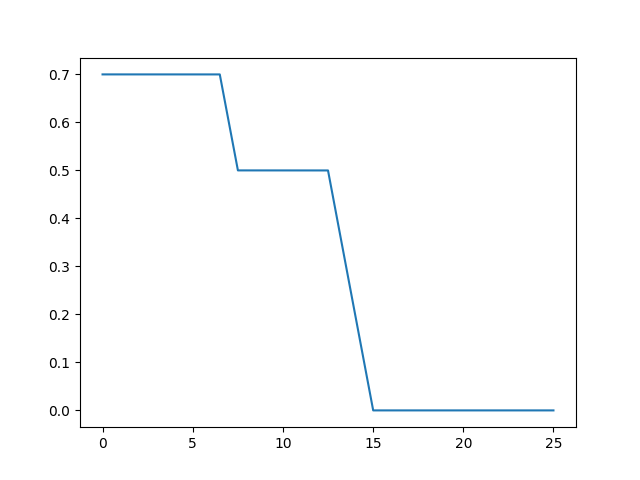
\includegraphics[width=.5\textwidth]{images/Eval_R87_V80.png}			
	\caption{Funci\'on resultante con par\'ametros 87 y 80 de ruido y volumen de la se\~nal, respectivamente, usando \emph{mamdani} y \emph{mom}. Se obtuvo como resultado $7.5$.}
	\label{fig:result}	
\end{figure}

\end{document}